\documentclass[landscape,a0,final]{a0poster}
\usepackage[dvipsnames,svgnames]{xcolor}
\usepackage{minted} %code highlighting, not working yet
\usepackage{tikzposter} % here most of the things are defined
% change parameters only after this line You can also start a new column with an arbitrary 
% x-coordinate by specifying explicitly the coordinate of the new block node as follows:
\usepackage[czech]{babel}
\usepackage[utf8]{inputenc}
\usepackage{wrapfig}
\usepackage{url}

%Used for better control on code display

\usepackage[margin=\margin cm, paperwidth=197cm, paperheight=100cm]{geometry}

% \setbackgrounddarkcolor{ForestGreen!70!black}
% \setbackgroundlightcolor{YellowGreen!90!}

% \setfirstcolor{YellowGreen!80!}
% \setsecondcolor{gray!80!}
% \setthirdcolor{red!80!black}

\title{From Water Dynamics to Rainfed Landscapes with GRASS GIS\bigskip}
\author{Yann Chemin$^1$, Martin van Brakel$^2$, Robyn Johnston$^1$, Jayne Curnow$^1$\\
\bigskip
\\ $^1$International Water Management Institute, $^2$CRP on Water, Land and Ecosystems (WLE)}

\usetemplate{1}
\setinstituteshift{1}

\setblocktitleheight{2}
\setblockspacing{1}

\begin{document}
\ClearShipoutPicture
\AddToShipoutPicture{\BackgroundPicture}
\noindent
\tikzstyle{every picture}+=[remember picture]
\begin{tikzpicture}
\initializesizeandshifts
\titleblock{120}{1}
% \setblocktitleheight{1}
\addlogo[north west]{(2,-1)}{9cm}{./svg_images/Grass_GIS.pdf}
\addlogo[north west]{(13,-3)}{19cm}{./svg_images/OSGeo_logo.pdf}
\addlogo[north east]{(-2,-4.5)}{30cm}{./images/CR10583_1wle-iwmi_logo}

%%%%%%%%%%%%%%%%%%%%%%%%%%%%%%%%%%%%%%%%%%%%%%%%%%%%%%%%%%%%%%%%%%%%%%%%%%%%%%%%
\blocknode{Abstract}{
\small \noindent Variability in water availability is a key determinant of risk and constraint to productivity in rainfed agricultural systems. Understanding the dynamics of water availability across both spatial and temporal scales is essential to managing water and optimize production. This research proposes to look at both the physical measurement of water availability and water user perceptions of landscapes and water availability.\newline\linebreak
\noindent Evapotranspiration makes up about three quarters of the transiting water in a landscape, it is composed of evaporation (water bodies, soil) and transpiration, the vegetation biomass growing quantity. This work will develop a methodology for defining landscapes based on water dynamics to be used at the interface of WLE research. The GRASS GIS [1] Imagery (i.*), Landscape (r.li.*) and Temporal (t.*) toolkits form the basis of the methodological development, from evapotranspiration modeling and landscape analysis to spatio-temporal analysis.\newline\linebreak
The methodology will be complemented by time series analysis spanning 14 years up to near real-time (2000-2014) of MODIS vegetation index data, capable of distinguishing seasonal and long term land use and land cover trends in these landscapes. This analysis will be developed into a routine that can be executed in open source GIS (GDAL [2] tools and GRASS GIS [1]), providing a robust and readily available application for monitoring medium to large scale land use and land cover change over any desired area.
}

%%%%%%%%%%%%%%%%%%%%%%%%%%%%%%%%%%%%%%%%%%%%%%%%%%%%%%%%%%%%%%%%%%%%%%%%%%%%%%%%
\blocknode{Transpiration and the search for rainfed landscapes}{
\smallskip
\begin{center}
	\begin{tabular}{c p{0.5\textwidth}}
	 \raisebox{-0.9\totalheight}{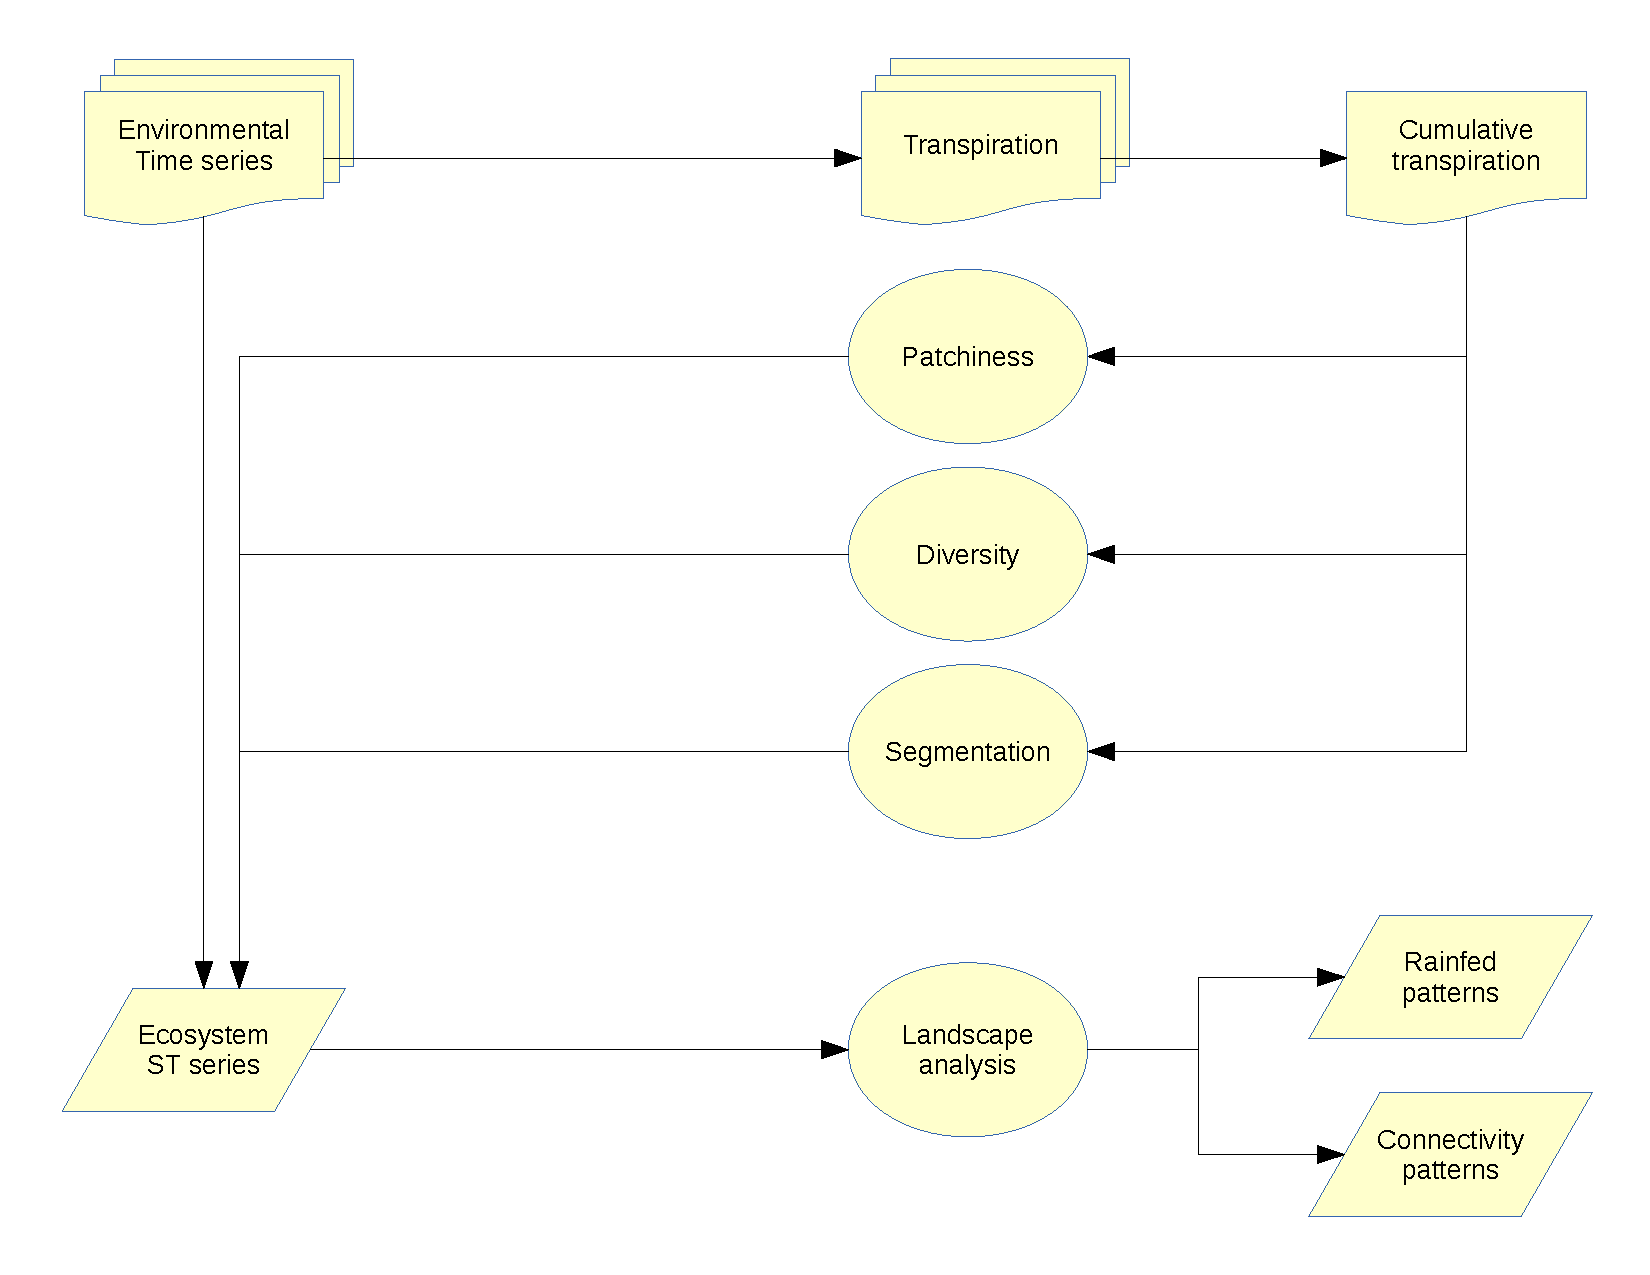
\includegraphics[width=0.45\textwidth]{./images/Yann_flowchart}}
	&
	The transpiration data is created from energy balance modelling [3] modules (i.eb.*, i.evapo.*) within GRASS GIS version 7, by partitioning the net radiation (r.sun) into soil heat flux (i.eb.soilheatflux), sensible heat flux (i.eb.h\_*) and the residual being the energy needed to evaporate water (i.eb.evapfr, i.eb.eta). This information is then fractionated into biotic (transpiration) and abiotic (evaporation) parts using vegetation fraction.\newline\linebreak
The accumulated transpiration (t.rast.aggregate) is subjected to Landscape analysis (r.li.*) for search of patchiness and diversity indices [4]. Further analysis of transpiration is also done with the object oriented classifier (i.segment) for spatiotemporal objects within the transpiration original dataset, the accumulated one and the Landscape indices, respectively.\newline
 	\end{tabular}\newline
\end{center}

}

%%%%%%%%%%%%%%%%%%%%%%%%%%%%%%%%%%%%%%%%%%%%%%%%%%%%%%%%%%%%%%%%%%%%%%%%%%%%%%%%
\getcurrentrow{box}
\coordinate (funkcionalita) at (box.south west);
\coordinate (funkcionalitaeast) at (box.east);
\coordinate (screenshot) at (box.north west);

\blocknodew[($(funkcionalita)+(20,-1)$)]{35}{References}{
\scriptsize
\begin{center}
\begin{tabular}{rp{0.9\textwidth}}
[1] & Neteler \& Bowman \&  Landa \& Metz, 2012. Environment \& Modeling Software, 31:124-130\\{}
[2] & GDAL, 2014. {\url {http://gdal.osgeo.org}}\\{}
[3] & Chemin, 2012. Chapter 19, DOI: 10.5772/23571 ({\url {http://bit.ly/16qJOep}})\\{}
[4] & McGarigal \& Marks, 1995. FRAGSTATS. USDA For. Serv. Gen. Tech. Rep. PNW-351.\\{}
[5] & Momsen \& Metz, 2012. GSoC project: Segmentation algorithm.
\end{tabular}
\end{center}
\smallskip
\hrulefill
\vspace{-5pt}

\begin{center}
\begin{tabular}{cp{0.9\textwidth}}
\begin{minipage}{0.15\textwidth}

\includegraphics[width=0.7in]{./images/iwmi_qr.pdf}
\end{minipage}

\begin{minipage}{0.3\textwidth}
\small {\url{www.iwmi.org}}
\end{minipage}

\begin{minipage}{0.15\textwidth}

\includegraphics[width=0.7in]{./images/grass_qr.pdf}
\end{minipage}

\begin{minipage}{0.3\textwidth}
\small {\url{grass.osgeo.org}}
\end{minipage}
\end{tabular}
\end{center}

\hrulefill
\vspace{14pt}
\begin{center}
\newcommand{\logowidth}{5em}
\newcommand{\logospace}{\hspace{0.1em}}
\noindent

\includegraphics[width=\logowidth]{./svg_images/public_domain_logo.pdf}
\raisebox{0.7\height}{\logospace 2013 GRASS Development Team}
\end{center}
}

\startsecondcolumn


%%%%%%%%%%%%%%%%%%%%%%%%%%%%%%%%%%%%%%%%%%%%%%%%%%%%%%%%%%%%%%%%%%%%%%%%%%%%%%%%
\blocknode{Temporal PCA-based classification}{
\smallskip
\begin{center}
	\begin{tabular}{c p{0.5\textwidth}}
	\raisebox{-0.9\totalheight}{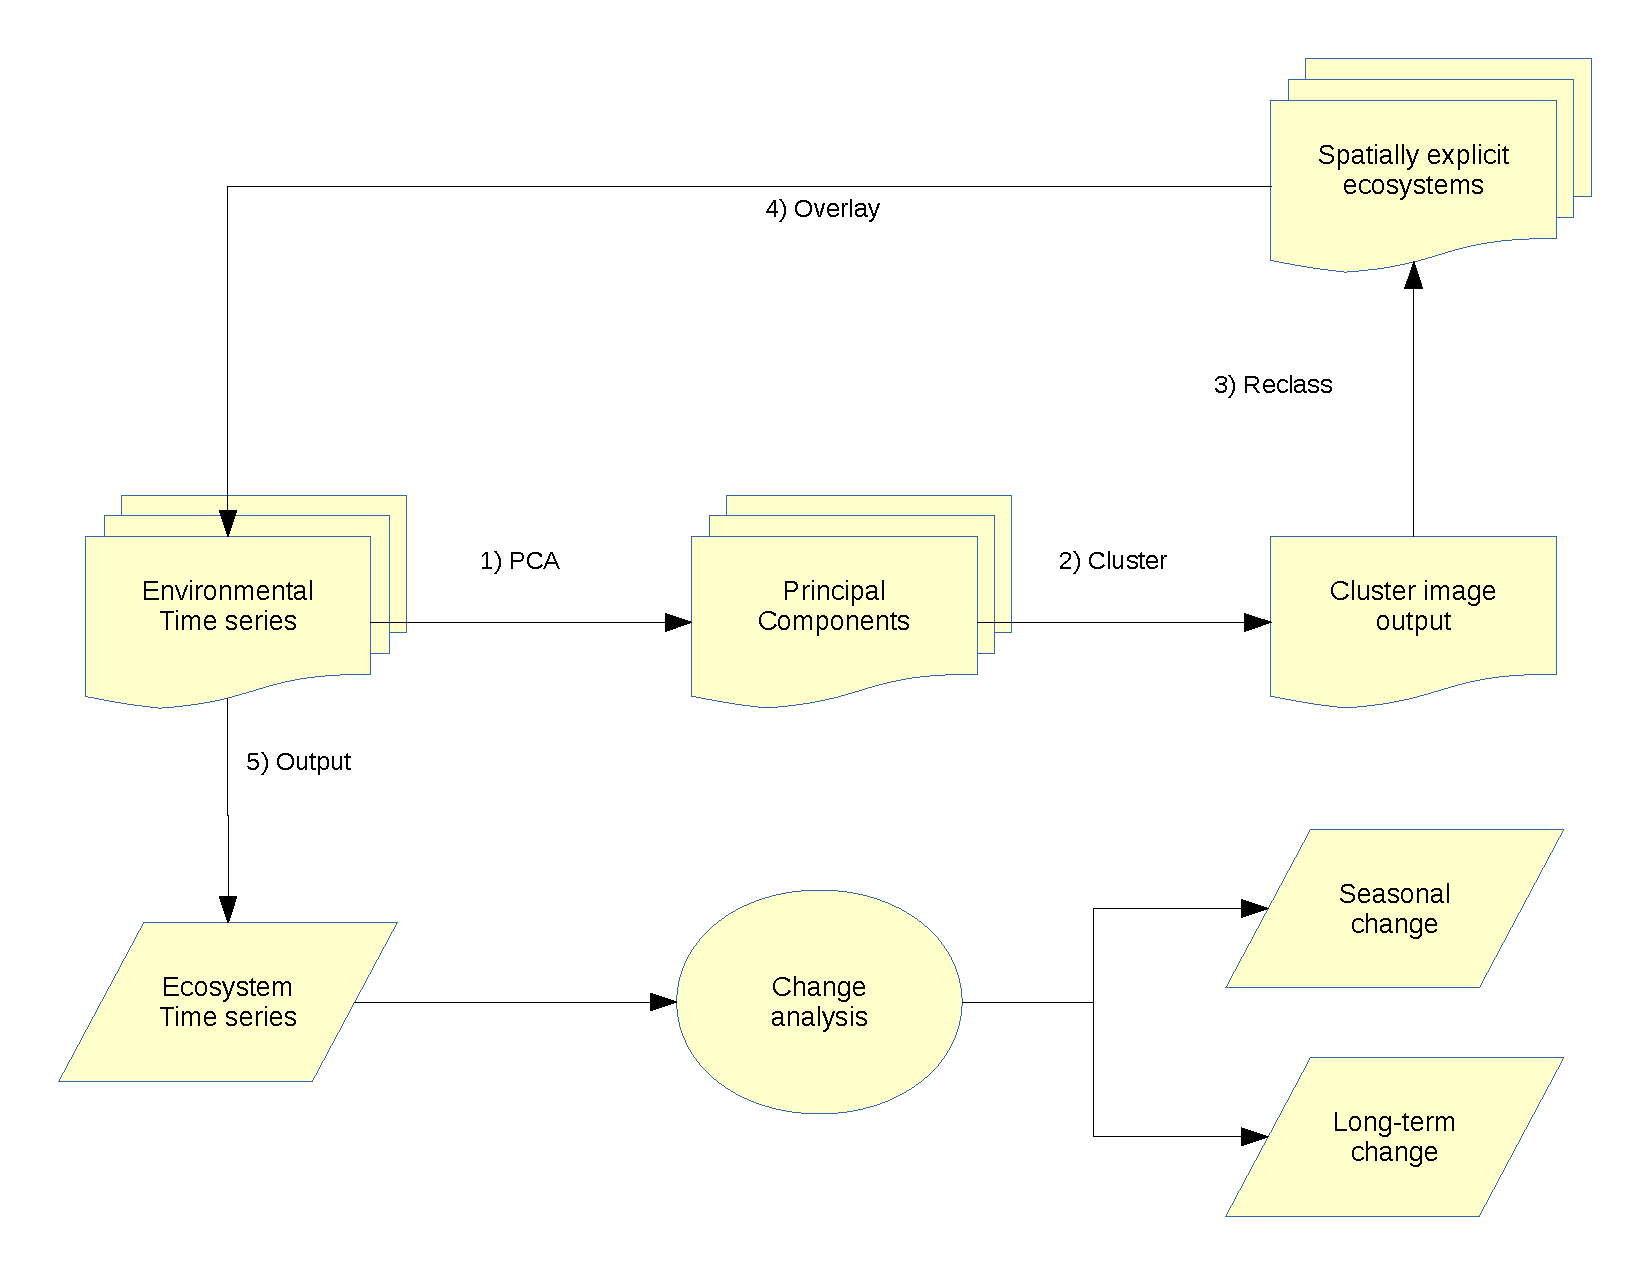
\includegraphics[width=0.45\textwidth]{./images/Martin_flowchart}}
	&
	A summary of the code needed to reach this point of analysis is here.\newline
	{\footnotesize \fontfamily{pcr}\selectfont i.group \textcolor{blue}{group}=pca\_group \textcolor{blue}{input}=\$(g.mlist \textcolor{blue}{type}=rast \textcolor{blue}{pattern}=*h28v07*EVI)\newline
	i.pca \textcolor{blue}{input}=pca\_group \textcolor{blue}{output\_prefix}=pca\_ \textcolor{blue}{percent}=99 --o\newline}
 	\end{tabular}\newline
\end{center}

%Minted version Not working (+ compile needs -shell-escape)
%\begin{minted}[frame=single,linenos,mathescape,fontsize=\small]{sh}
%	i.group group=pca_group input=$(g.mlist type=rast pattern=*h28v07*EVI)
%	i.pca input=pca_group output_prefix=pca_ percent=99 --o
%\end{minted}
}

%%%%%%%%%%%%%%%%%%%%%%%%%%%%%%%%%%%%%%%%%%%%%%%%%%%%%%%%%%%%%%%%%%%%%%%%%%%%%%%%
\blocknode{Temporal PCA-based classification}{
Balaaaaaaaaaaaaaaaaaaaaaaaaaaaaaaaaaaaaaaaaaaaaaaaaaaaaaaaaaaaaaaaaaaaaaaaaaaaa
aaaaaaaaaaaaaaaaaaaaaaaaaaaaaa\newline
\begin{center}
	\begin{tabular}{cc}
 	\raisebox{-0.5\totalheight}{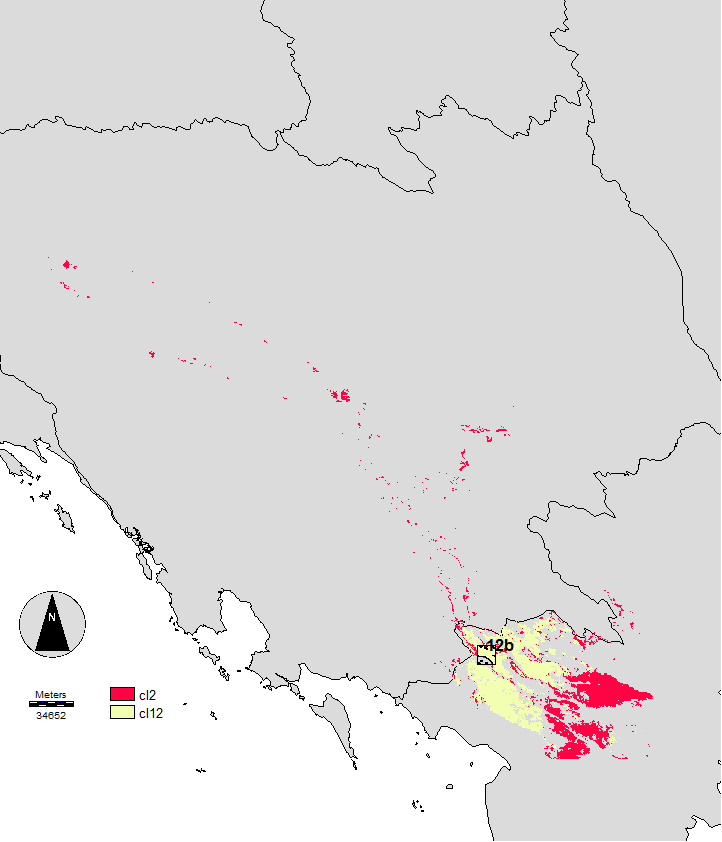
\includegraphics[width=0.45\textwidth]{./images/MSUBAS_MD}}
 	& 
 	\begin{tabular}{c}
 	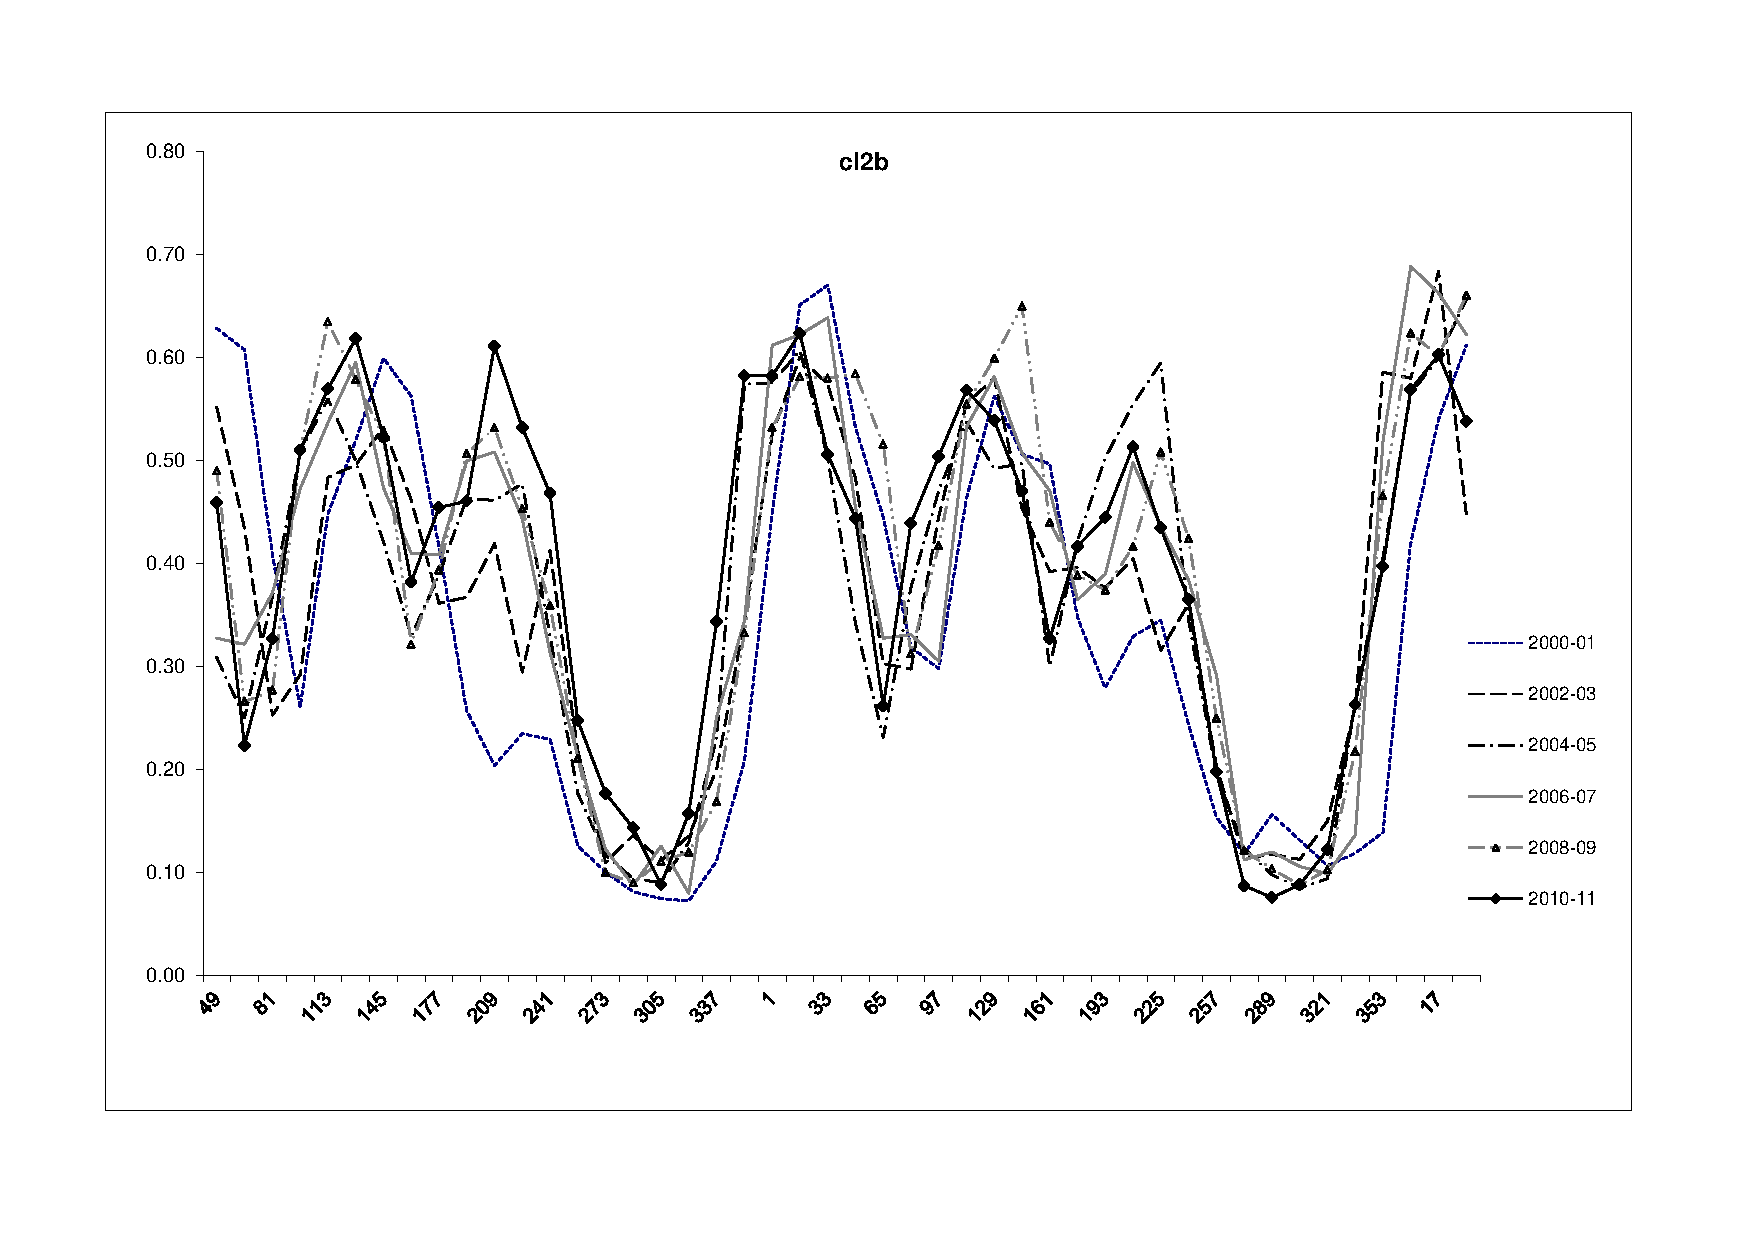
\includegraphics[width=0.45\textwidth]{./images/cl2_DoY}\\
 	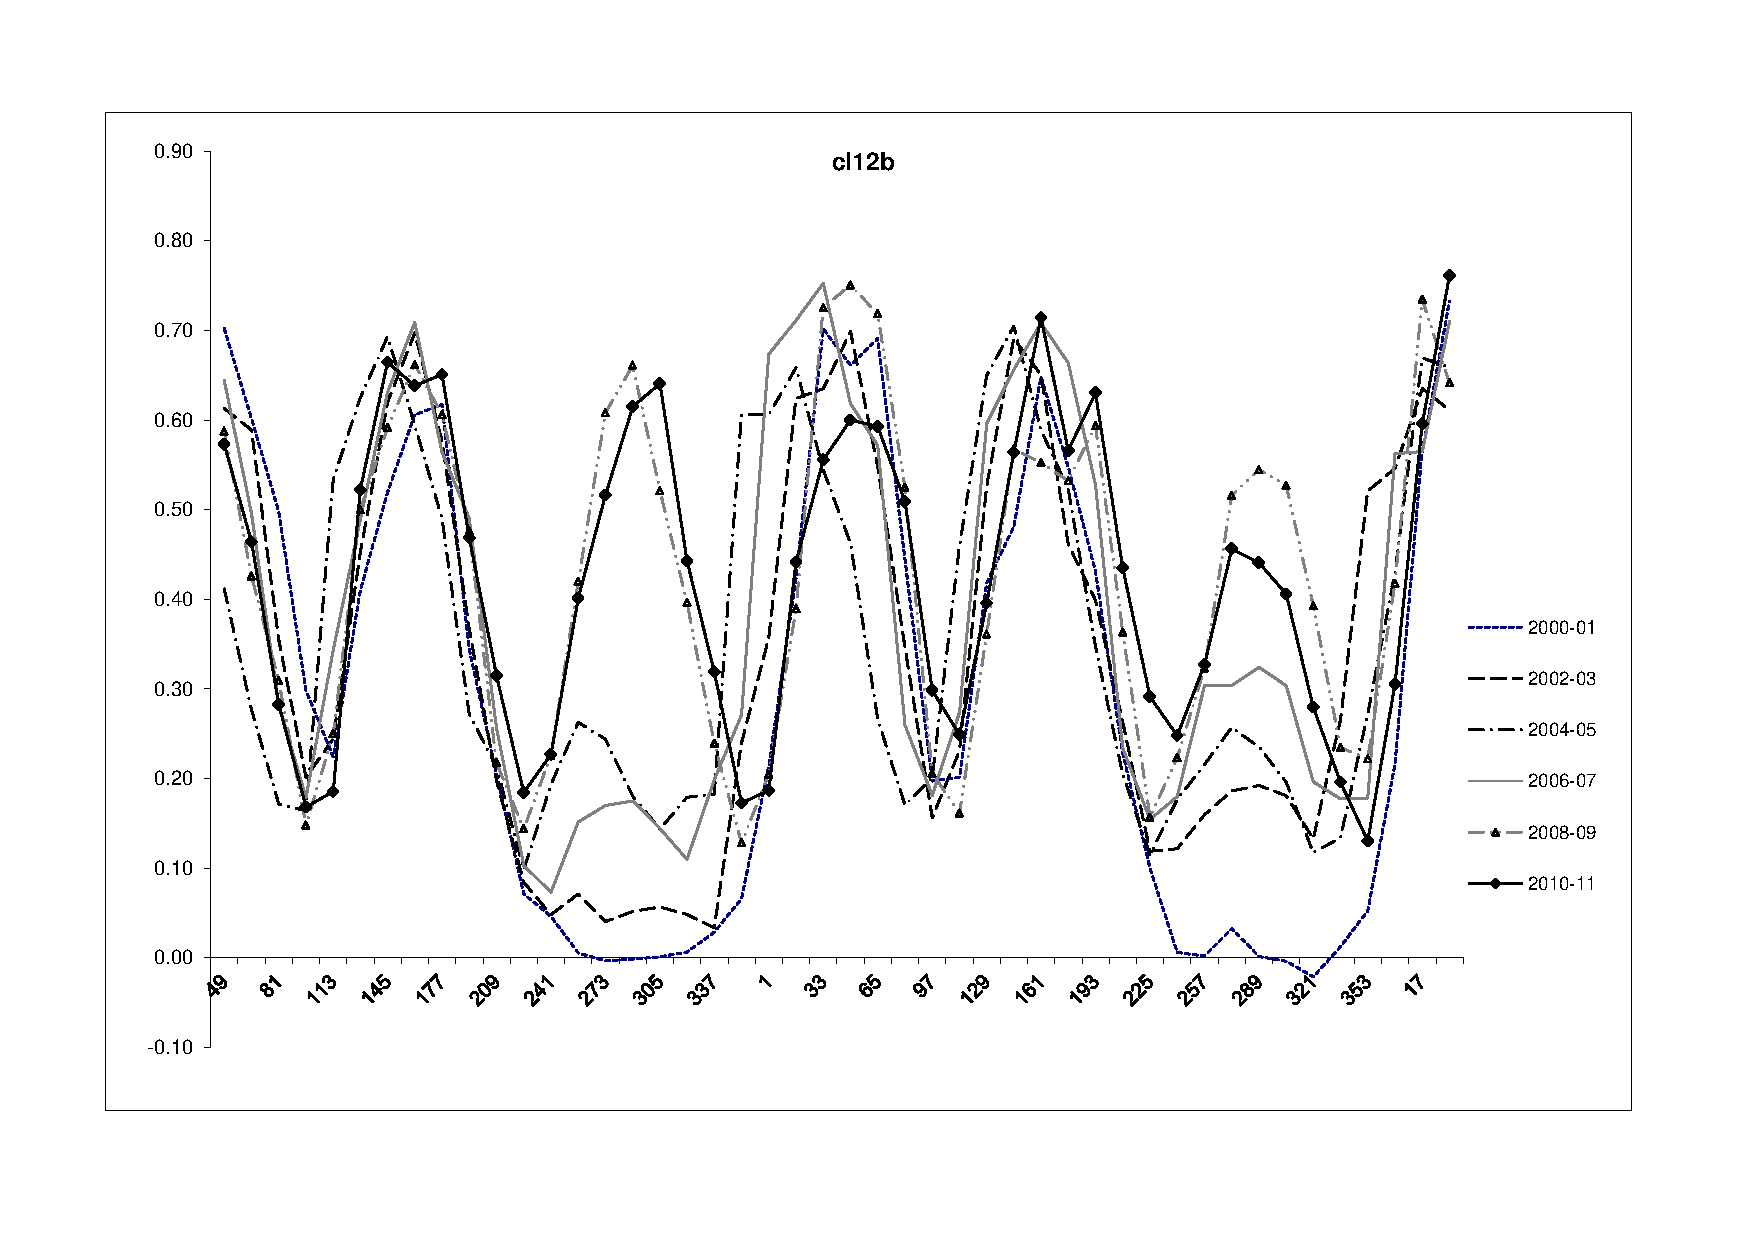
\includegraphics[width=0.45\textwidth]{./images/cl12_DoY}
	\end{tabular}
	\end{tabular}\newline
	Figure 2: Temporal 
\end{center}

}

\startthirdcolumn

%%%%%%%%%%%%%%%%%%%%%%%%%%%%%%%%%%%%%%%%%%%%%%%%%%%%%%%%%%%%%%%%%%%%%%%%%%%%%%%%
\blocknode{Temporal patterns of recession cropping \& natural vegetation}{

\begin{center}
	\begin{tabular}{cc}
	\raisebox{-0.7\totalheight}{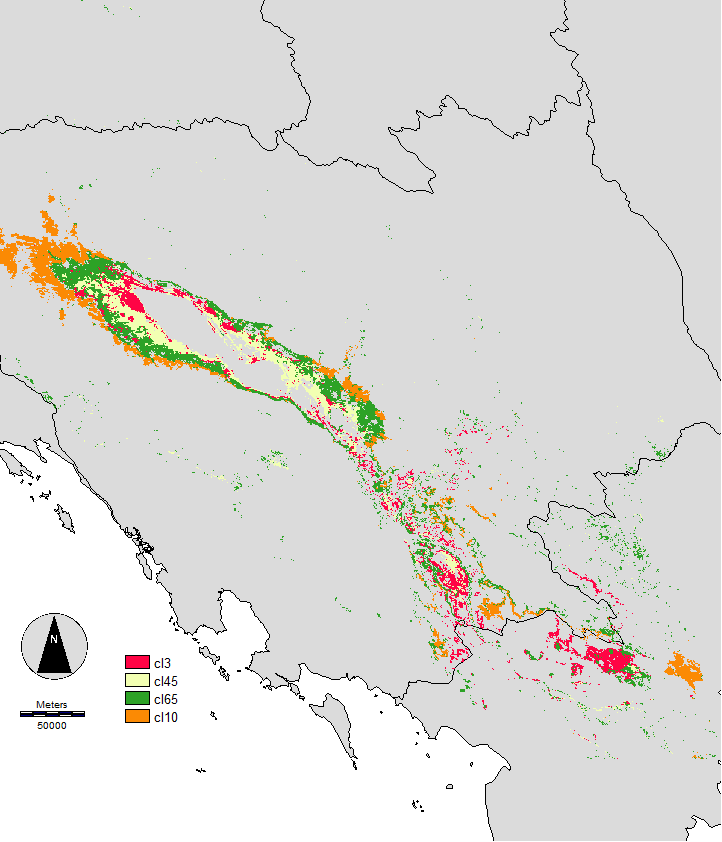
\includegraphics[width=0.45\textwidth]{./images/MSUBAS_TS}}
	&
	\begin{tabular}{c}
 	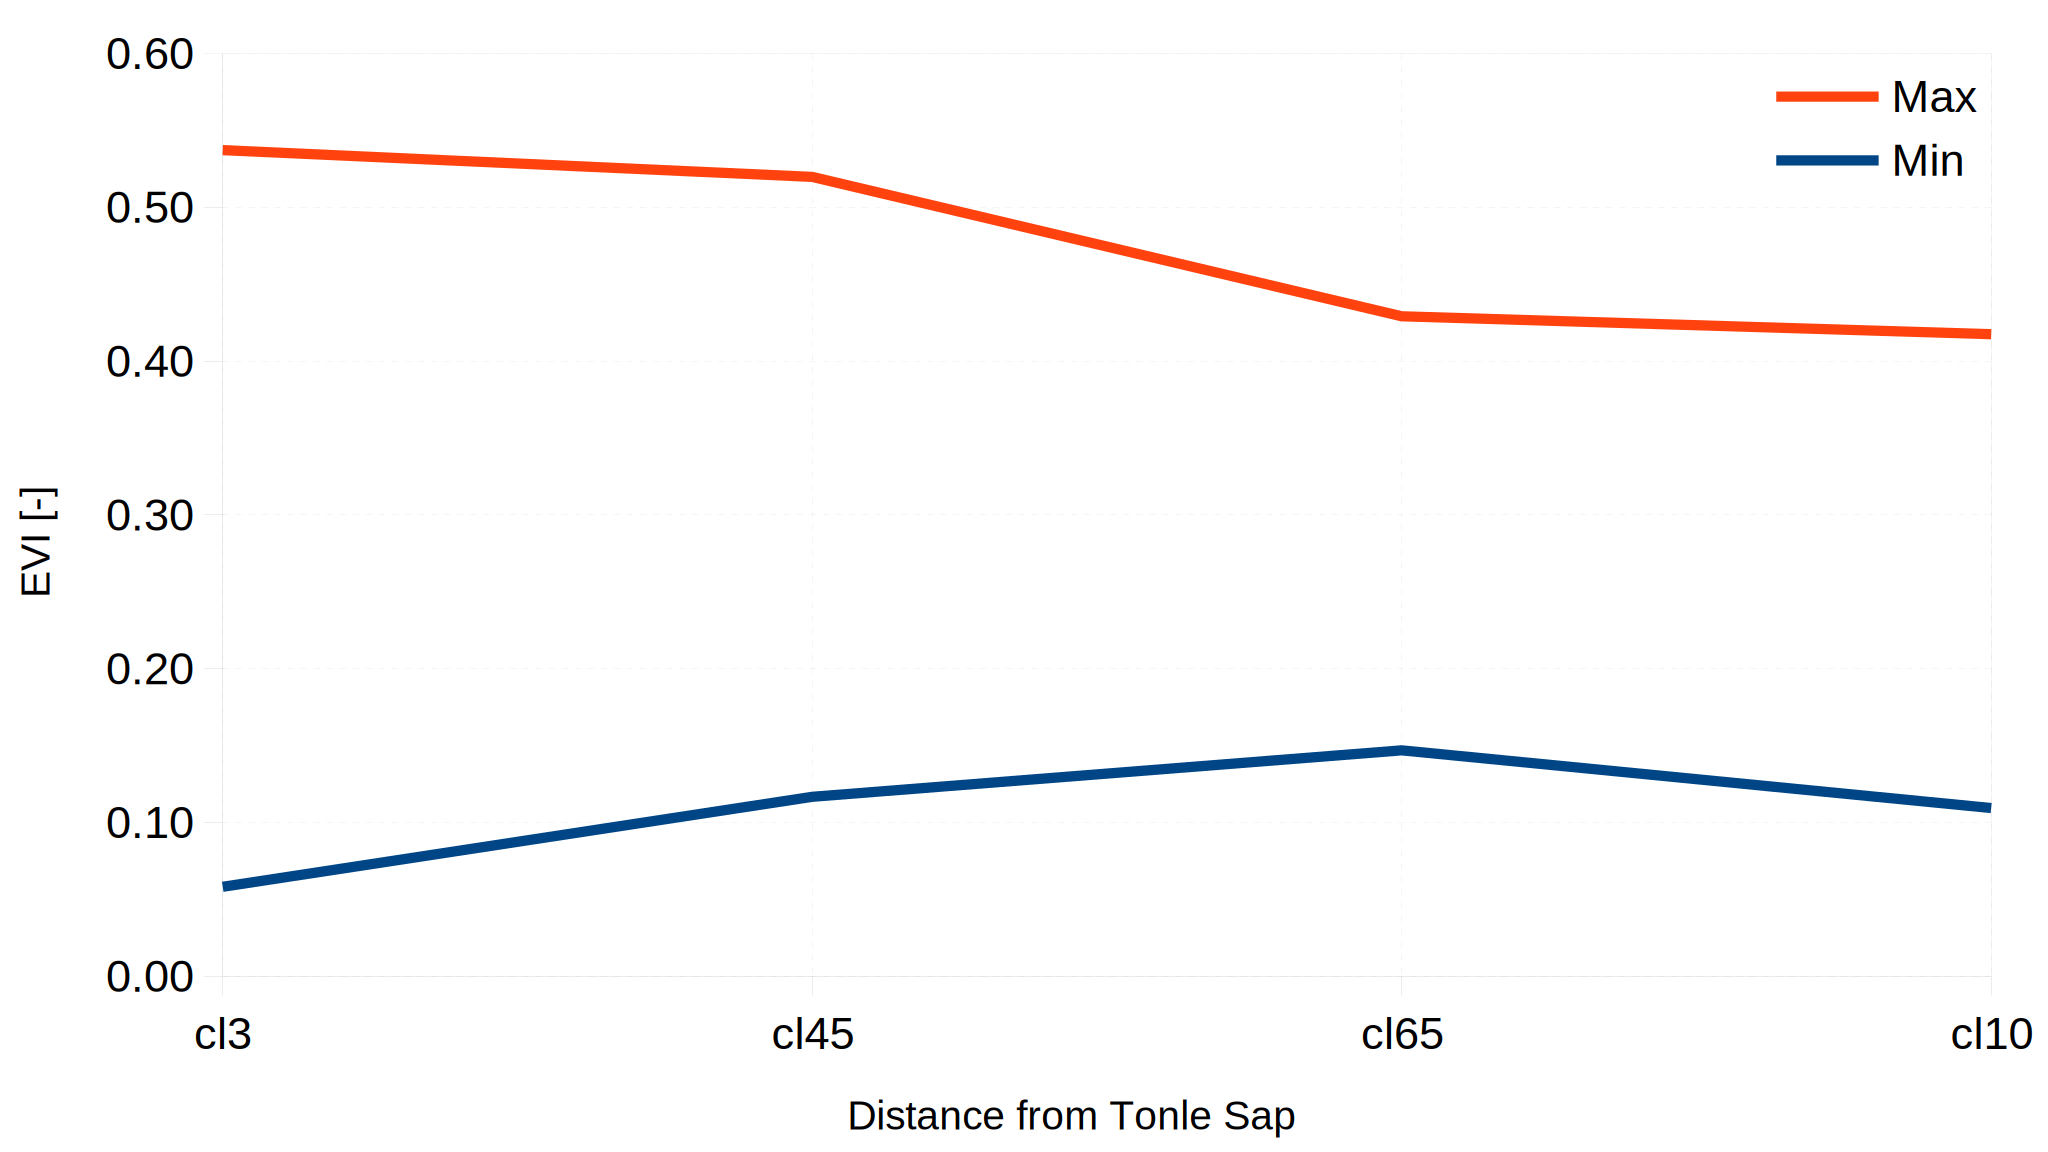
\includegraphics[width=0.45\textwidth]{./svg_images/EVI_distance_from_tonle_sap}\\
	bllaaaaaaaaaaaaaaaaaaaaaaaaaaaaaaaaaaaaaaaaaa
	\end{tabular}
 	\end{tabular}\newline
\end{center}

}

%%%%%%%%%%%%%%%%%%%%%%%%%%%%%%%%%%%%%%%%%%%%%%%%%%%%%%%%%%%%%%%%%%%%%%%%%%%%%%%%
\blocknode{Recession cropping \& natural vegetation}{
\begin{center}
	\begin{tabular}{cc}
 	\begin{tabular}{c}
 	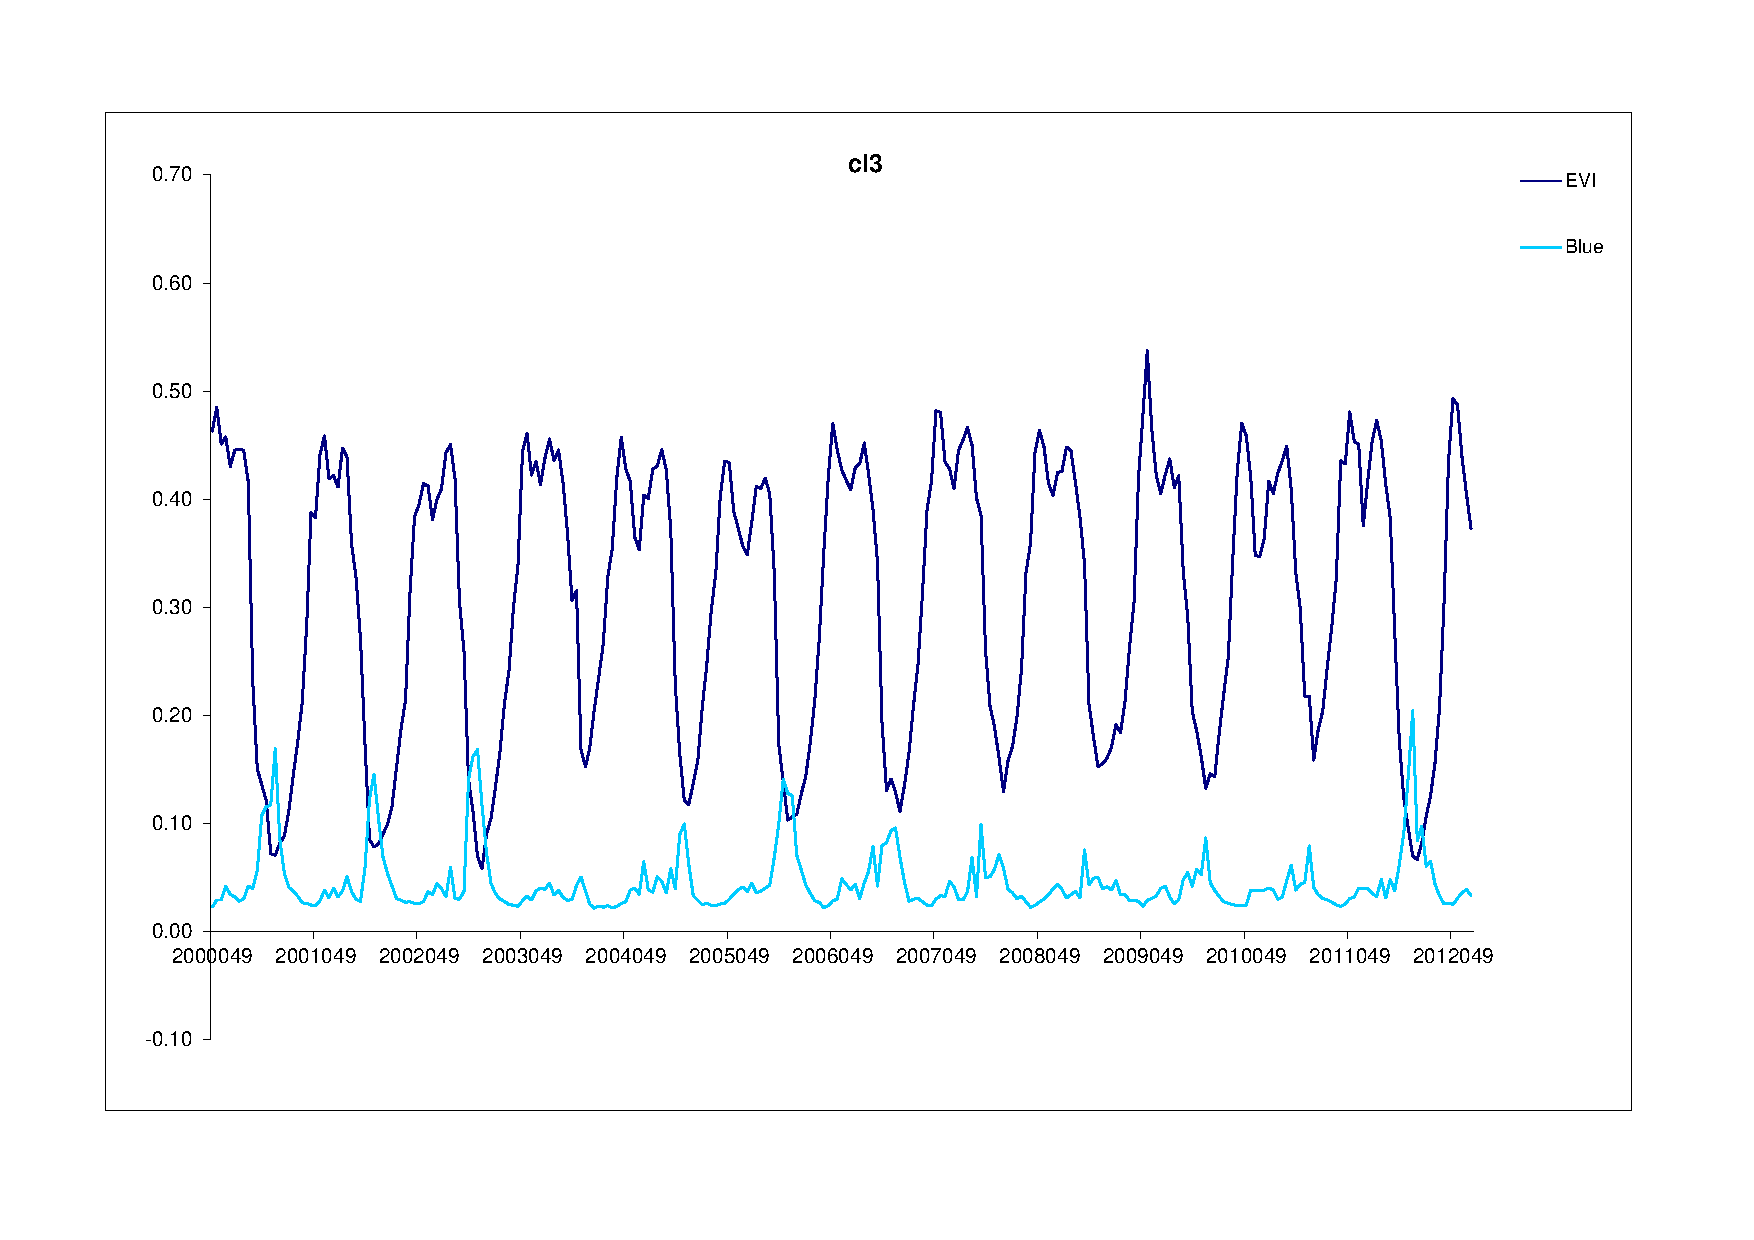
\includegraphics[width=0.5\textwidth]{./images/cl3_avg}\\
 	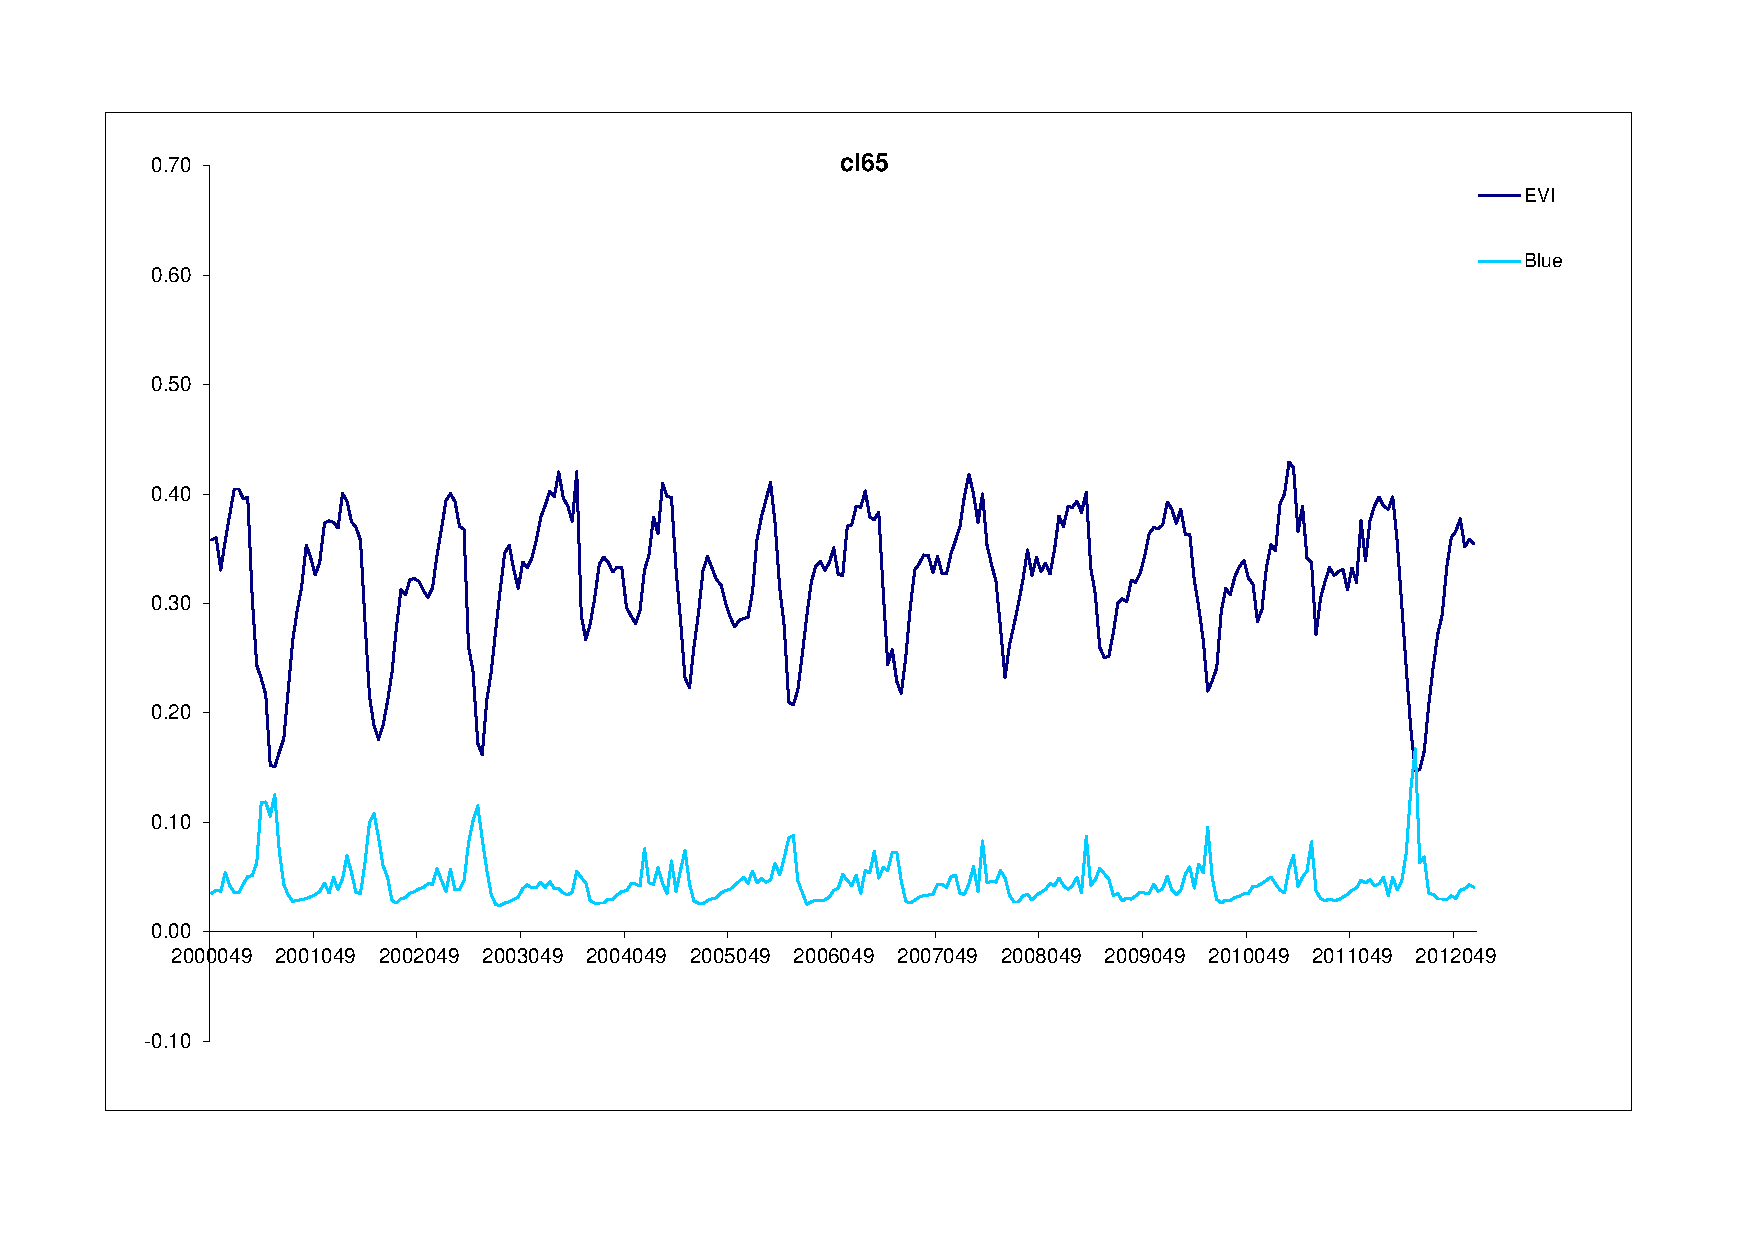
\includegraphics[width=0.5\textwidth]{./images/cl65_avg}
	\end{tabular}
 	& 
 	\begin{tabular}{c}
 	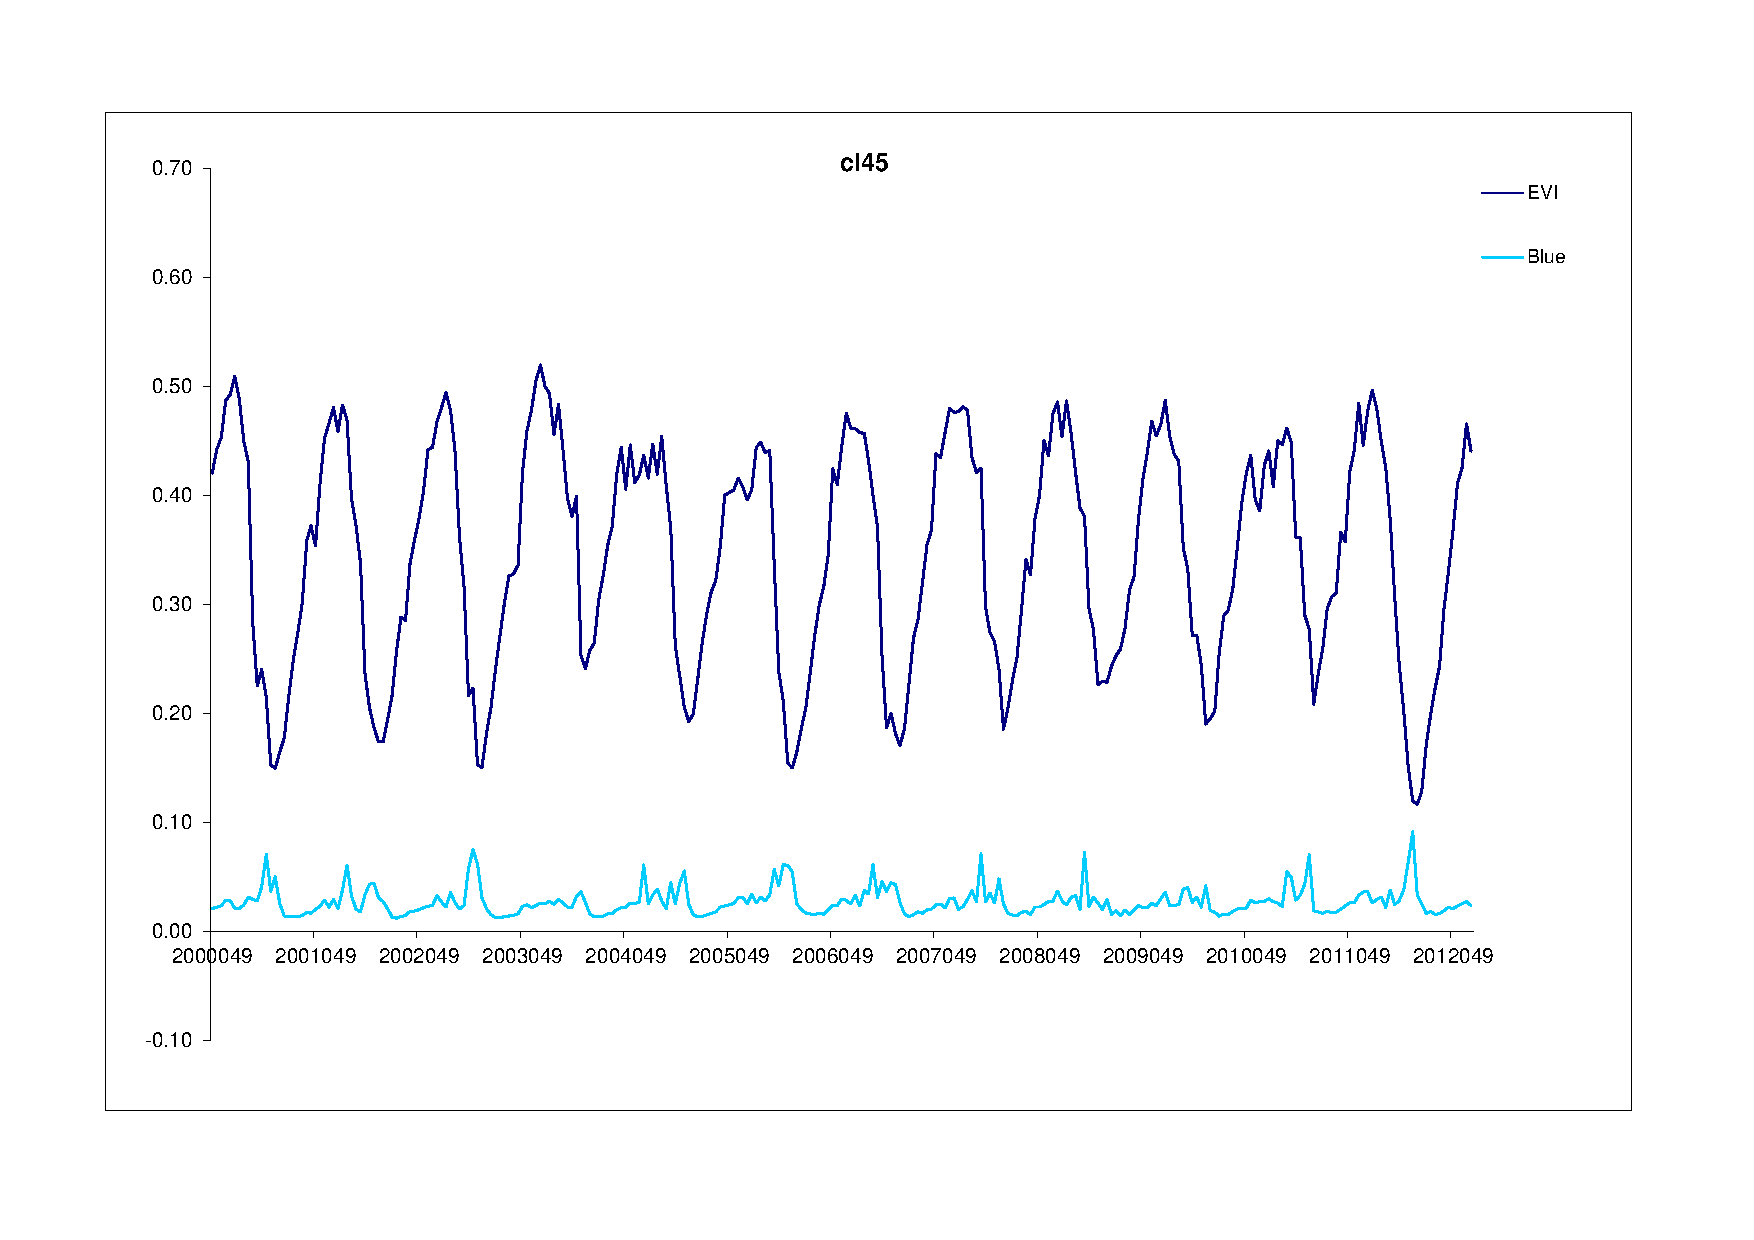
\includegraphics[width=0.5\textwidth]{./images/cl45_avg}\\
 	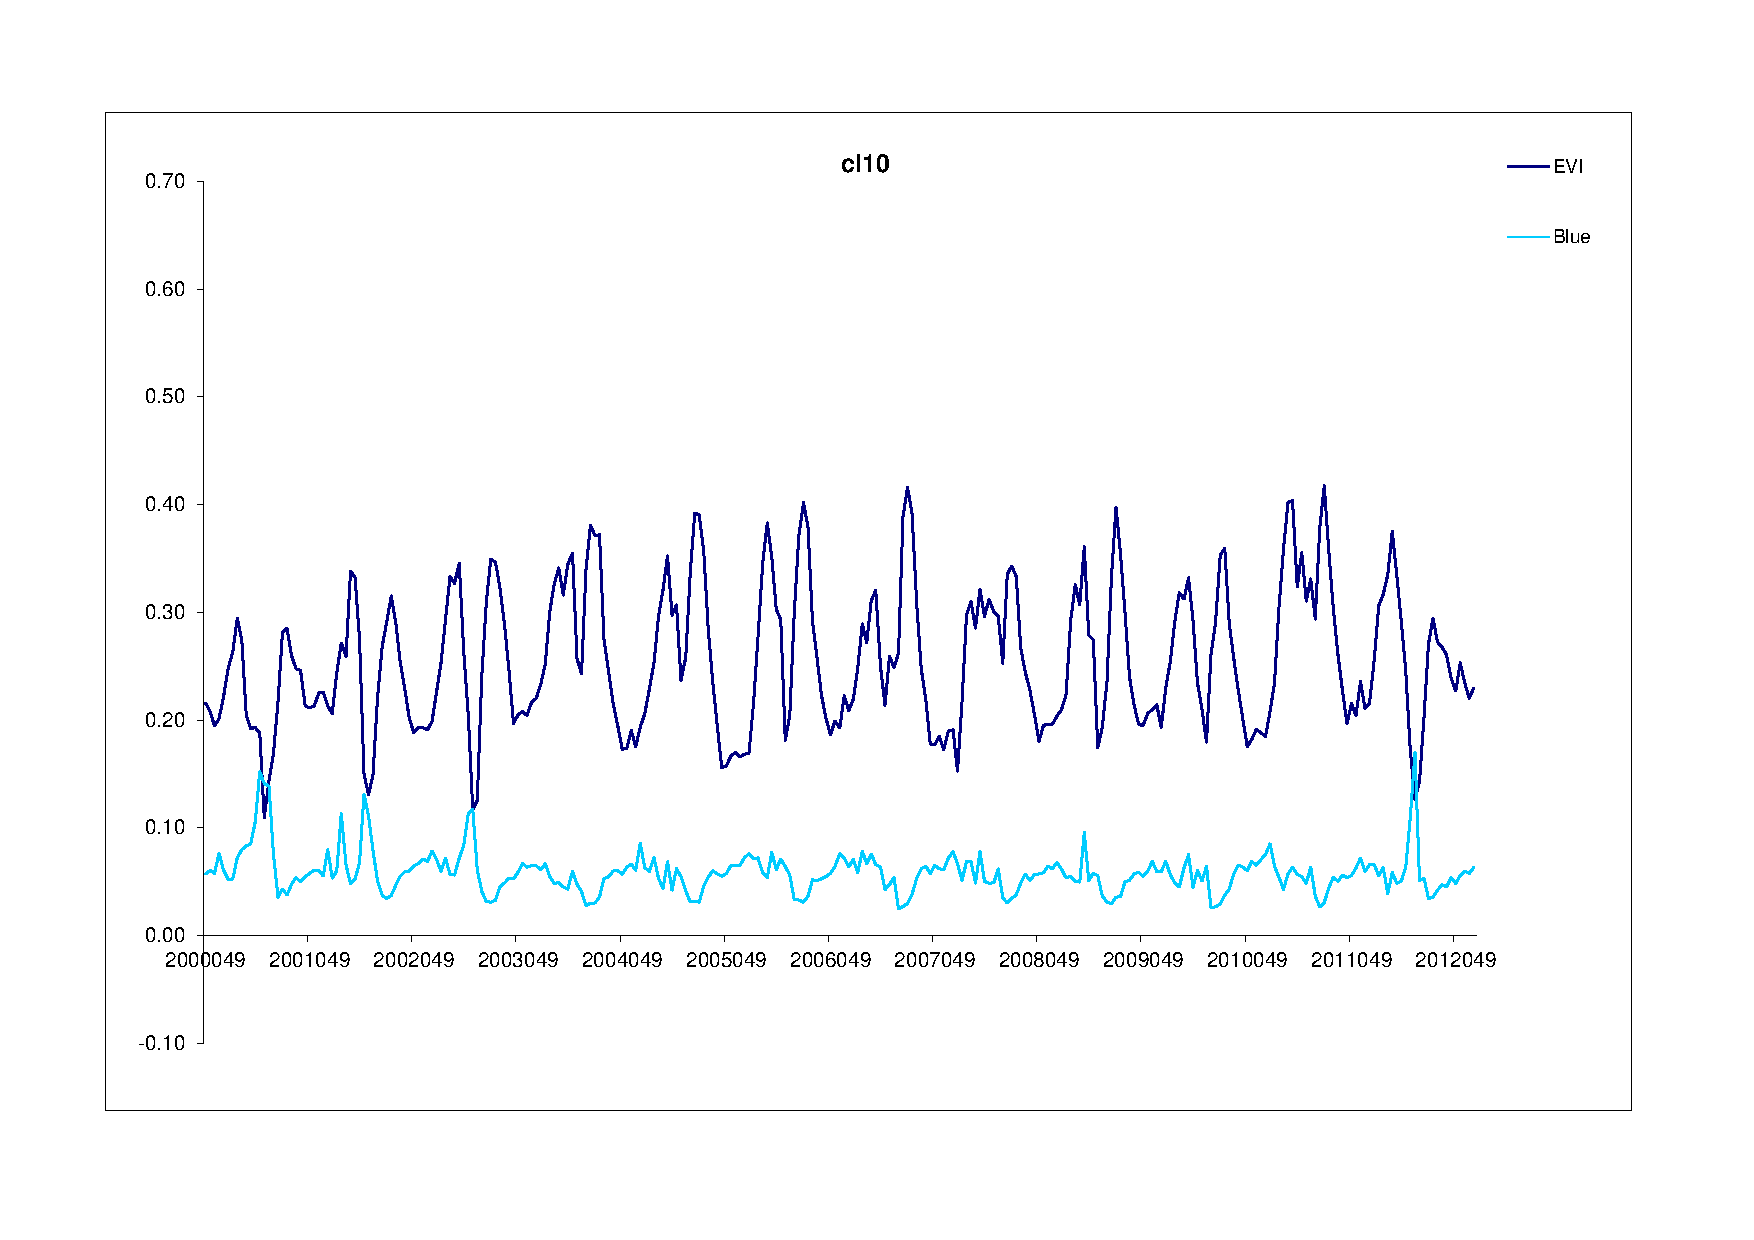
\includegraphics[width=0.5\textwidth]{./images/cl10_avg}
	\end{tabular}
	\end{tabular}\newline
\end{center}

}



\startfourthcolumn

%%%%%%%%%%%%%%%%%%%%%%%%%%%%%%%%%%%%%%%%%%%%%%%%%%%%%%%%%%%%%%%%%%%%%%%%%%%%%%%%
\blocknode{Euclidian Distance plotting}{
\smallskip

\begin{center}
	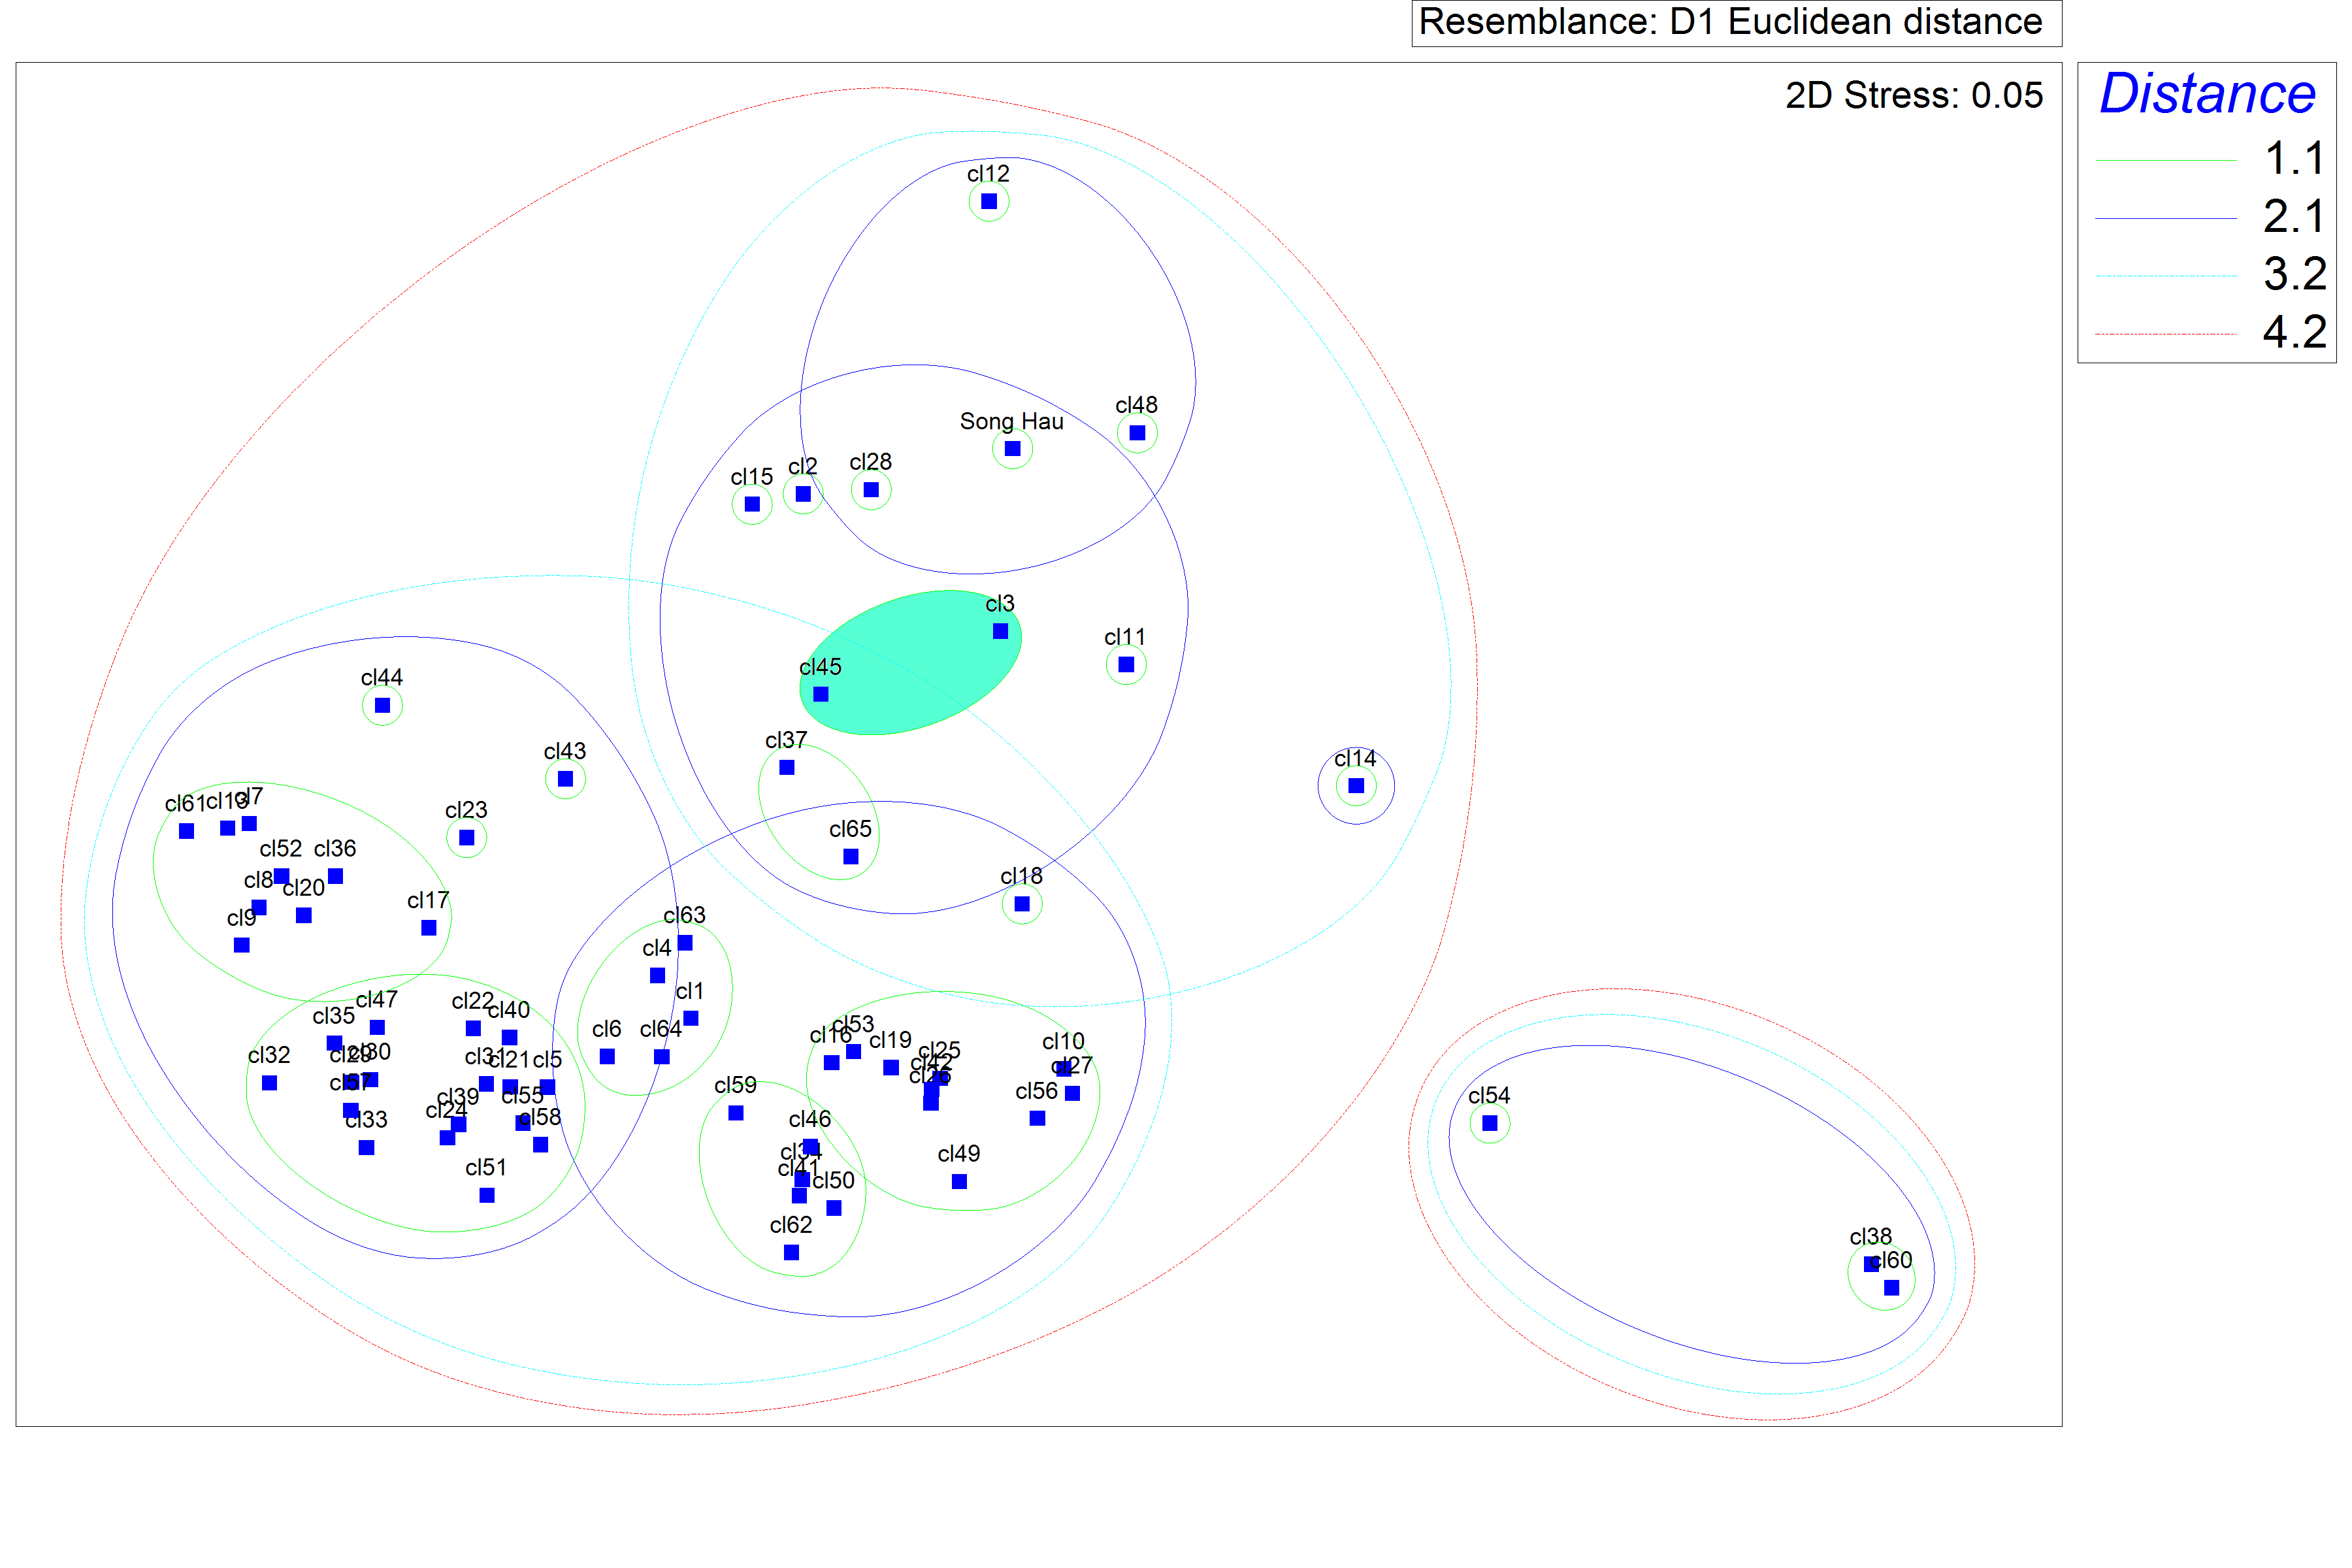
\includegraphics[width=0.75\textwidth]{./images/msubas65}
\end{center}

}

\end{tikzpicture}

\end{document}
